\chapter{Introducción}
\label{cap:introduccion}
\setcounter{page}{1}

La evolución tecnológica ha provocado una transformación radical en nuestra forma de vivir, trabajar y relacionarnos desempeñando la tecnología un papel 
fundamental en el avance de la sociedad e impulsando una serie de innovaciones que se extienden desde la invención de la rueda hasta la era digital contemporánea. 
Por ejemplo, los ordenadores empezaron siendo grandes máquinas que ocupaban habitaciones enteras que requerían una gran cantidad de energía y mantenimiento. Hoy en día, los ordenadores
son dispositivos ligeros y eficientes que pueden realizar múltiples cálculos por segundos que se utilizan en diferentes ramas de las ingenierías como la informática, telecomunicaciones y,
por supuesto, la robótica. \newline

La robótica, en particular, se destaca como una de las ramas de la tecnología que más impacto significativo ha tenido. Estos avances han facilitado numerosas tareas mejorando la eficiencia 
y la capacidad de enfrentar desafíos complejos dando pie a nuevas posibilidades en nuestro entorno. Un ejemplo de ello puede ser la robótica aérea con el uso de los drones, 
demostrando ser desafiantes y valiosos en la inspección de áreas de difícil acceso, el mapeo de terrenos, la realización de entregas, la navegación autónoma o la captura 
de imágenes desde alturas elevadas. Su versatilidad y su capacidad para poder operar en entornos peligrosos o inaccesibles para los seres humanos los convierten 
en herramientas fundamentales en campos como la agricultura, la seguridad, la investigación medioambiental y la logística. 

\section{La robótica}
\label{sec:enfoquesrobotica}
Como mencionamos anteriormente, entre las diversas ramas de la tecnología, la robótica se destaca como una de las más prometedoras. Apareciendo como disciplina durante la década de los años 60, 
la robótica ha tenido un cambio asombroso  pasando de ser simples máquinas programables a sistemas inteligentes capaces de aprender y adaptarse 
a su entorno teniendo avances en diversas disciplinas de la ingeniería, como la informática, la inteligencia artificial, la ingeniería de control, la mecánica, 
la electricidad y la electrónica. 
Los robots de hoy en día no solo tienen la capacidad de realizar tareas programadas y repetitivas, sino que también tienen la capacidad de interactuar con su entorno, 
tomar decisiones basadas en la información sensorial y aprender de sus experiencias. Este avance en la robótica nos ha permitido tener una definición más precisa de lo que es 
la robótica moderna, definiendo la robótica como ciencia interdisciplinaria encargada de la creación, funcionamiento, estructuración, fabricación y uso de los robots. 
Esta definición incluye no solo los componentes mecánicos y eléctricos, sino que también los algoritmos de control, los sensores que les permiten recopilar
datos de su entorno y los sistemas que procesan esta información y toman decisiones.

\begin{figure} [H]
  \begin{center}
    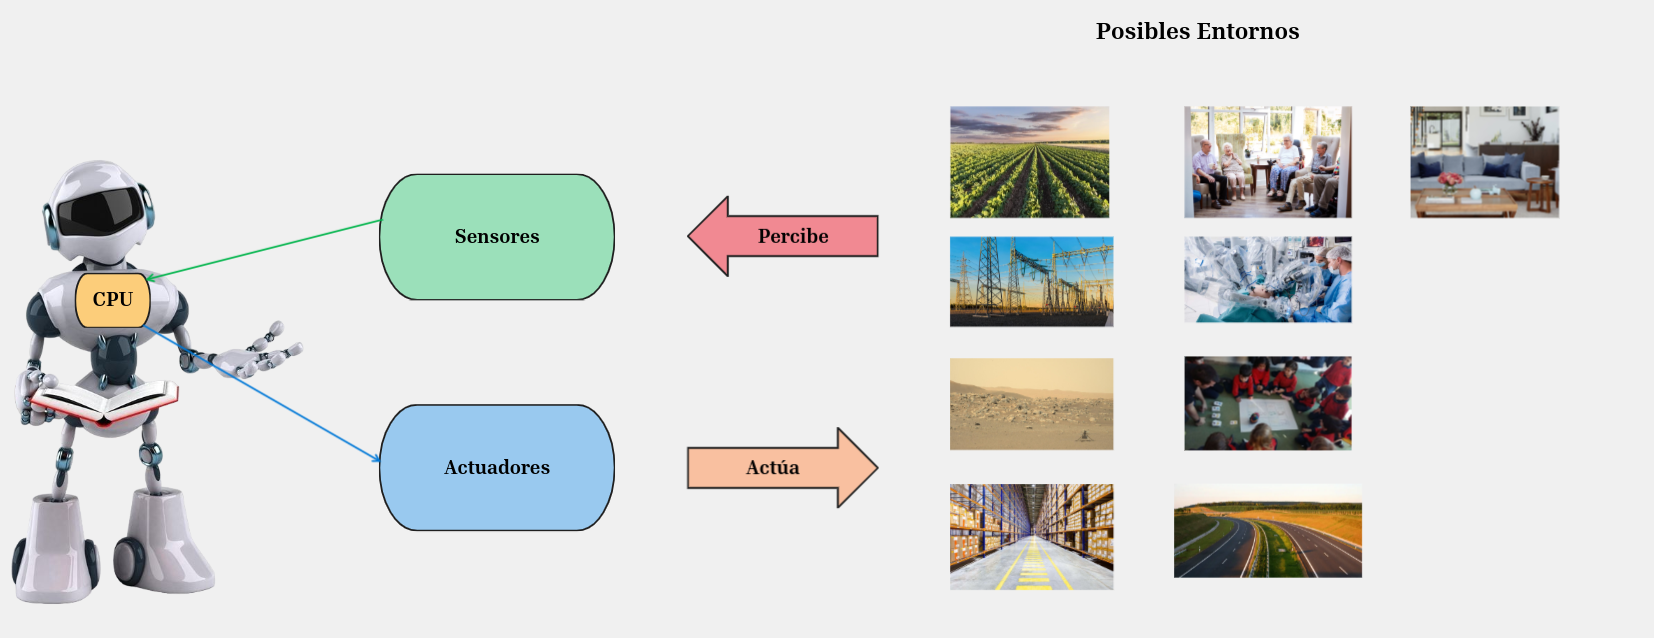
\includegraphics[scale=0.25]{figs/introducción/robot.png}
  \end{center}
  \caption{Definición de robot.}
  \label{fig:robot}
\end{figure}\

La capacidad de los robots para aprender y adaptarse a su entorno abre nuevas oportunidades en campos como la medicina, la exploración lunar, la asistencia personal, la automatización industrial, etc. 
Además de abrir nuevas aplicaciones y tareas como puede ser la navegación autónoma, la detección de objetos o 
la manipulación de objetos con sensores táctiles y de fuerza, dichas tareas que pueden realizar, pueden ser peligrosas, delicadas, sucias o monótonas 
(conocidas como las 4D's: dull,dirty, dangerous and dear)\footnote{\url{https://www.forbes.com/sites/bernardmarr/2017/10/16/the-4-ds-of-robotization-dull-dirty-dangerous-and-dear/?sh=40bb6cec3e0d}}


 % etiqueta para luego referenciar esta sección
 \subsection{Enfoques de control en el mundo de la robótica}
 \label{sec:enfoquesrobotica}
A lo largo de la evolución de la robótica, han surgido tres enfoques fundamentales para el diseño y la operación de robots. Cada uno de estos enfoques presentan diferentes
formas de interactuar y operar robots, con sus riesgos, características y aplicaciones únicas. 

\subsubsection{Teleoperación}
\label{sec:subseccion}

La teleoperación surge de la necesidad de manipular objetos o realizar tareas en entornos complejos, peligrosos y distantes para el ser humano. Desde la historia, el ser humano
ha utilizado una variedad de herramientas para ampliar su capacidad de manipulación como palos utilizados para caer la fruta madura de un árbol. Con el tiempo, se desarrollaron 
dispositivos más complejos, como pinzas que permitían manipular piezas o alcanzar objetos de difícil acceso facilitando el trabajo para el operario. En la era moderna, la teleoperación
ha estado evolucionando hasta el punto de incluir sistemas robóticos robustos que pueden ser controlados a distancia, permitiendo al operario poder realizar
tareas en entornos peligrosos e inaccesibles para el ser humano como puede ser la exploración espacial, la medicina o la inspección nuclear.
La intervención del operador humano en los sistemas de teleoperación de robots es imprescindible, debe ser capaz de poder interpretar los datos sensoriales que proporciona el robot, así como de 
tomar decisiones robustas y precisas dependiendo de la situación. Esto conlleva tener una capacidad de realizar múltiple tareas simultáneamente adpatandose a situaciones imprevistas. \newline

Hoy en día, la teleoperación de robots tiene variedad de aplicaciones. Una de ellas puede ser la exploración espacial, en donde se utiliza la teleoperación
como técnica de manipulación remota como el Sojourner Rover. Como se muestra en la figura \ref{fig:Sojourner}, El Sojourner Rover\footnote{\url{https://www.astronomy.com/space-exploration/sojourner-nasas-first-mars-rover/}} 
es un pequeño robot móvil compuesto por 6 ruedas creado por los científicos de la NASA para estudiar 
la superficie de Marte con la capacidad de enviar imágenes en directo y realizar análisis del terreno del planeta. Gracias a sus ruedas podía moverse por terrenos rocosos y de difícil acceso
ya que estaban equipadas materiales como de aluminio y acero inoxidable. \newline

\begin{figure} [H]
  \begin{center}
    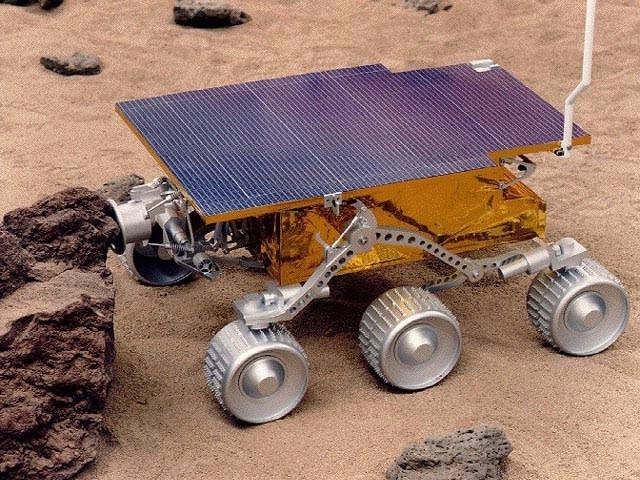
\includegraphics[scale=0.4]{figs/introducción/Sojourner.jpg}
  \end{center}
  \caption{Sojourner Rover}
  \label{fig:Sojourner}
\end{figure}\

Con esta misión espacial se pudo probar como era el entorno marciano con técnicas realizadas en los laboratorios de la NASA demostrando que se podía realizar una teleoperación en 
el espacio abriendo el camino a futuros rovers como el Spirit, Opportunity y más\footnote{\url{https://spaceplace.nasa.gov/mars-spirit-opportunity/sp/}}. \newline

A pesar de ser un buen enfoque en cuanto a controlar un robot, presenta sus propias limitaciones, como la dependencia de una conexión continua y confiable entre
el operario y el robot. Si la conexión se interrumpe, el control del robot podría perderse desembocando situaciones de grave peligro. Otro tipo de limitación puede ser la carga
cognitiva que puede tener el operario al controlar el robot, ya que el operario debe permanecer concentrado monitorizando y controlando el robot de manera constante.
Lo último puede conducir a errores humanos, especialmente durante operaciones de larga duración, lo que hace interesante tener otro tipo de enfoque de control.

\subsubsection{Robótica Semiautónoma}
\label{sec:subseccion}
Los robots pueden realizar tareas de forma independiente siguiendo instrucciones preprogramadas o tomando decisiones en tiempo real, este enfoque se le conoce como autonomía o semi-autonomía, 
siendo la diferencia que en el enfoque semi-autónomo todavía existe parte de teleoperación en el robot. Este enfoque permite que los robots puedan ser autónomos para poder
percibir su entorno y en la toma de decisiones, pero con el handicap de que un operario humano pueda controlarlo para poder ajustar parámetros, cambiar objetivos o intervenir 
en caso de emergencia. \newline

Aunque los robots semi-autónomos puedan tomar decisiones en tiempo real, a menudo siguen instrucciones preprogramadas o reciben ordenes de un operario humano, esta toma de decisiones
puede incluir elegir la ruta más eficiente para navegar por un entorno peligroso como puede ser el robot submarino llamado Nereus como se ilustra en la figura \ref{fig:Nereus}. El Nereus\footnote{\url{https://www.bbc.com/mundo/ciencia_tecnologia/2009/06/090603_1541_nereus_robot_mar_mr}} 
es un vehículo submarino semi-autónomo que puede ser manejado por control remoto que entro en servicio en el año 2009, su propósito fue explorar la Fosa de las Marianas, específicamente el Abismo Challenger (es el punto más
profundo conocido en los océanos). Fue manejado mediante control remoto por pilotos que se encontraban en un barco en la superficie, aunque el Nereus también podía cambiar al modo
de vehículo autónomo pudiendo navegar libremente adaptándose a las condiciones del entorno sin intervención humana directa. \newline

\begin{figure} [H]
  \begin{center}
    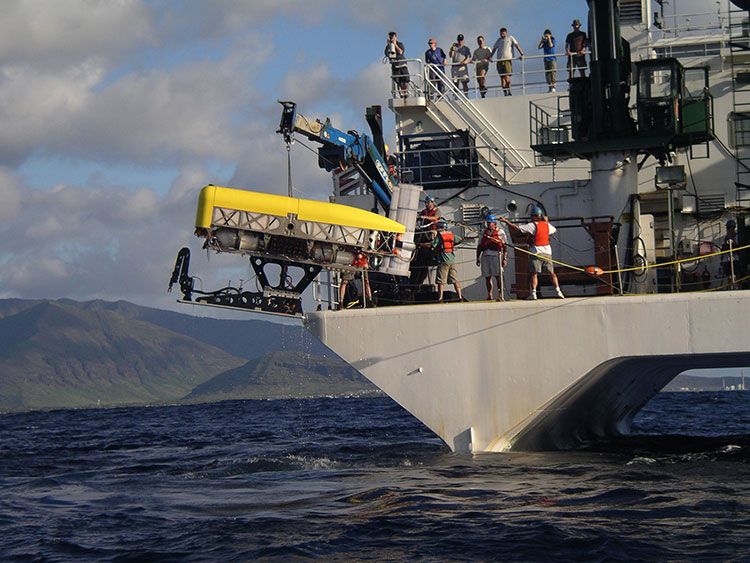
\includegraphics[scale=0.4]{figs/introducción/nereus.jpg}
  \end{center}
  \caption{Nereus}
  \label{fig:Nereus}
\end{figure}\

Lamentablemente, en 2014 durante una misión, el robot Nereus sufrió un colapso estructural y se perdió en el fondo del océano. A pesar de esta perdida, los datos que se pudieron
recopilar en este robot submarino siguen siendo una fuente de conocimiento sobre las profundidades marinas. Este ejemplo de robot semi-autónomo demuestra que se pueden realizar 
tareas en entornos peligrosos sin poner en riesgo la vida humana aunque tenga control por un operario\footnote{\url{https://www.elperiodico.com/es/ciencia/20140512/famoso-sumergible-nereus-pierde-fondo-mar-3271389}}. 

En cuanto a las debilidades de la robótica semiautonóma, estos robots 
aún requieren intervención humana para tareas complejas o situaciones imprevistas, aunque la dependencia del operario sea menor todavía sigue siendo significativa. 
Se debe garantizar la seguridad y la fiabilidad de estos sistemas semi-autónomos, cualquier fallo en la autonomía del robot 
o en la intervención humana puede tener consecuencias peligrosas y asimismo de que los algoritmos perceptivos y de control de los robots semi-autónomos deben ser eficientes y 
robustos ante situaciones cambiantes.

\subsubsection{Robótica Autónoma}
\label{sec:subseccion}

La robótica autónoma consiste en desarrollar robots que sean capaces de operar y realizar tareas de forma independiente sin la intervención de un ser humano. En contraste con los 
robots teleoperados, este tipo de robots necesitan un comportamiento más robusto y preciso para realizar tareas independientes basándose en la percepción del entorno 
y en la toma de decisiones autónomas.
El concepto de automía en los sistemas robóticos se esta convirtiendo en un área de investigación activa y en rápido desarrollo. Los avances en inteligencia artificial (IA), visión 
artificial, aprendizaje automático han facilitado la creación de robots autónomos capaces de llevar a acabo amplias variedades de tareas en entornos no estructurados y cambiantes. 
Uno de los grandes desafíos que enfrenta la robótica autónoma es cómo el robot puede realizar la percepción del entorno, identificando y comprendiendo objetos y situaciones de manera
precisa y en tiempo real. \newline

Por ejemplo, como se muestra en la figura \ref{fig:Rega}, el robot autónomo parecido a un helicóptero diseñado por investigadores suizos es capaz de realizar tareas de 
rescate y búsqueda en los Alpes suizos\footnote{\url{https://www.swissinfo.ch/spa/ciencia/drones-suizos-al-rescate/46203902}}. Este dron autónomo puede llegar a escanear amplias zonas de montaña y reconocer personas en tierra de manera autónoma mediante
cámaras y algoritmos de aprendizaje automático desarrollados por la ETH Zúrich. Facilitando las tareas de rescate al equipo de rescate Rega siguiendo rutas
predefinidas sin intervención humana directa localizando a personas atrapadas o en peligro en áreas remotas o accidentadas.

\begin{figure} [H]
  \begin{center}
    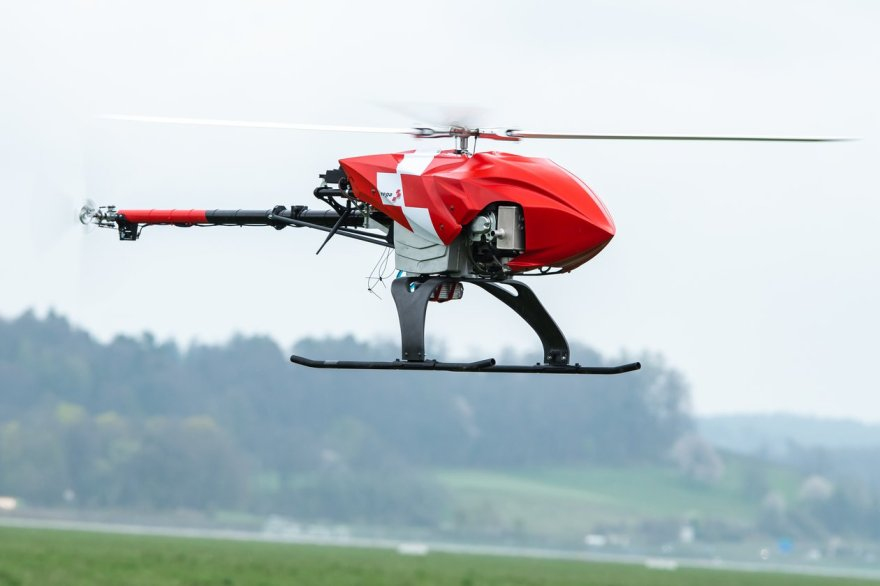
\includegraphics[scale=0.4]{figs/introducción/Rega.jpg}
  \end{center}
  \caption{El dron de rescate Rega}
  \label{fig:Rega}
\end{figure}\

\section{Robótica aérea}
\label{sec:subseccion}

Dentro del campo de la robótica aérea tenemos los drones. Podemos definir un dron, como vehículo aéreo no tripulado (UAV), es un tipo de aeronave que puede operar sin la 
necesidad de un piloto humano a bordo. Estos dispositivos pueden ser controlados remotamente por un operador humano o navegar autonómicamente incorporando software 
en su sistema. 
El origen de los drones se remonta a la Primera Guerra Mundial con el biplano Kettering Bug.
Este era un torpedo no tripulado de 240 kg (con una envergadura de 4,5 m, una longitud de
3,8 m y una altura de 2,3 m)\footnote{\url{https://www.nationalmuseum.af.mil/Visit/Museum-Exhibits/Fact-Sheets/Display/Article/198095/kettering-aerial-torpedo-bug/}} era propulsado por un motor alternativo. Podía volar de
forma autónoma hasta un punto específico, donde soltaba sus alas y caía en “caída libre”\footnote{\url{https://daytonunknown.com/2023/06/30/the-kettering-bug-the-worlds-first-drone/}}.
Avanzando en la historia, en 1935 se desarrolló el DH.82 Queen Bee\footnote{\url{https://dronewars.net/2014/10/06/rise-of-the-reapers-a-brief-history-of-drones/}}. Éste era un blanco aéreo sin piloto que era controlado por radio. De hecho, parece que el término “dron” se originó a partir del nombre, que se refiere a la abeja macho que realiza un vuelo en busca de la abeja reina y luego fallece. \newline

Durante la Segunda Guerra Mundial, quizás el más conocido fue el V-1 "Flying Bomb"\footnote{\url{https://migflug.com/jetflights/the-v1-flying-bomb/}} , el primer misil
de crucero operativo del mundo, en donde su sistema de guía prestablecido incluía una brújula magnética que monitorizaba un auto-piloto con giroscopios. También en este periodo, destacaremos el \textit{Proyect Aphrodite} \cite{Aphrodite}, fue un programa que tenía como objetivo convertir bombarderos en bombas voladoras no tripuladas que eran controladas por radio. Más adelante estos bombarderos no tripulados se utilizaron para volar a través de nubes de hongo
después de las pruebas nucleares. \newline

Destacando más UAVs, tenemos la familia Teledyne Ryan Firebee/Firefly\footnote{\url{https://www.designation-systems.net/dusrm/m-34.html}}, estos sistemas generalmente se lanzaban 
desde el aire y se recuperaban mediante una combinación de paracaídas y helicópteros. El Lockheed D-21 fue uno de los sistemas más impresionantes durante la Guerra Fría. 
Este UAV fue propulsado por estatorreactor con velocidades mayores que Mach 3\footnote{\url{https://www.marchfield.org/aircraft/unmanned/d-21-drone-lockheed/}} . 
En la Edad Moderna, destacamos El Condor \cite{CondorUAV}, fue el primer UAS en utilizar navegación GPS y tecnología de aterrizaje automático y el Predactor\footnote{\url{https://www.airforce-technology.com/projects/predator-uav/?cf-view}}. 
En la época dorada, gracias a los avances anteriores se pudo desarrollar sistemas militares esenciales que han demostrado su valor y el desarrollo de vehículos aéreos no 
tripulados pequeños (small UAV). Este ultimo ha despertado un gran interés significativo resaltando como puntos de entrega al mercado civil ya que con sus cargas útiles
reducidas pueden ser portátiles y tener un coste menor. \newline

En la figura \ref{f:Drones} se ilustra la historia de los drones que se ha comentado anteriormente, desde la Primera Guerra Mundial hasta la actualidad.

\begin{figure}[H]
  \begin{center}
    \subfigure[Kettering Bug]{
     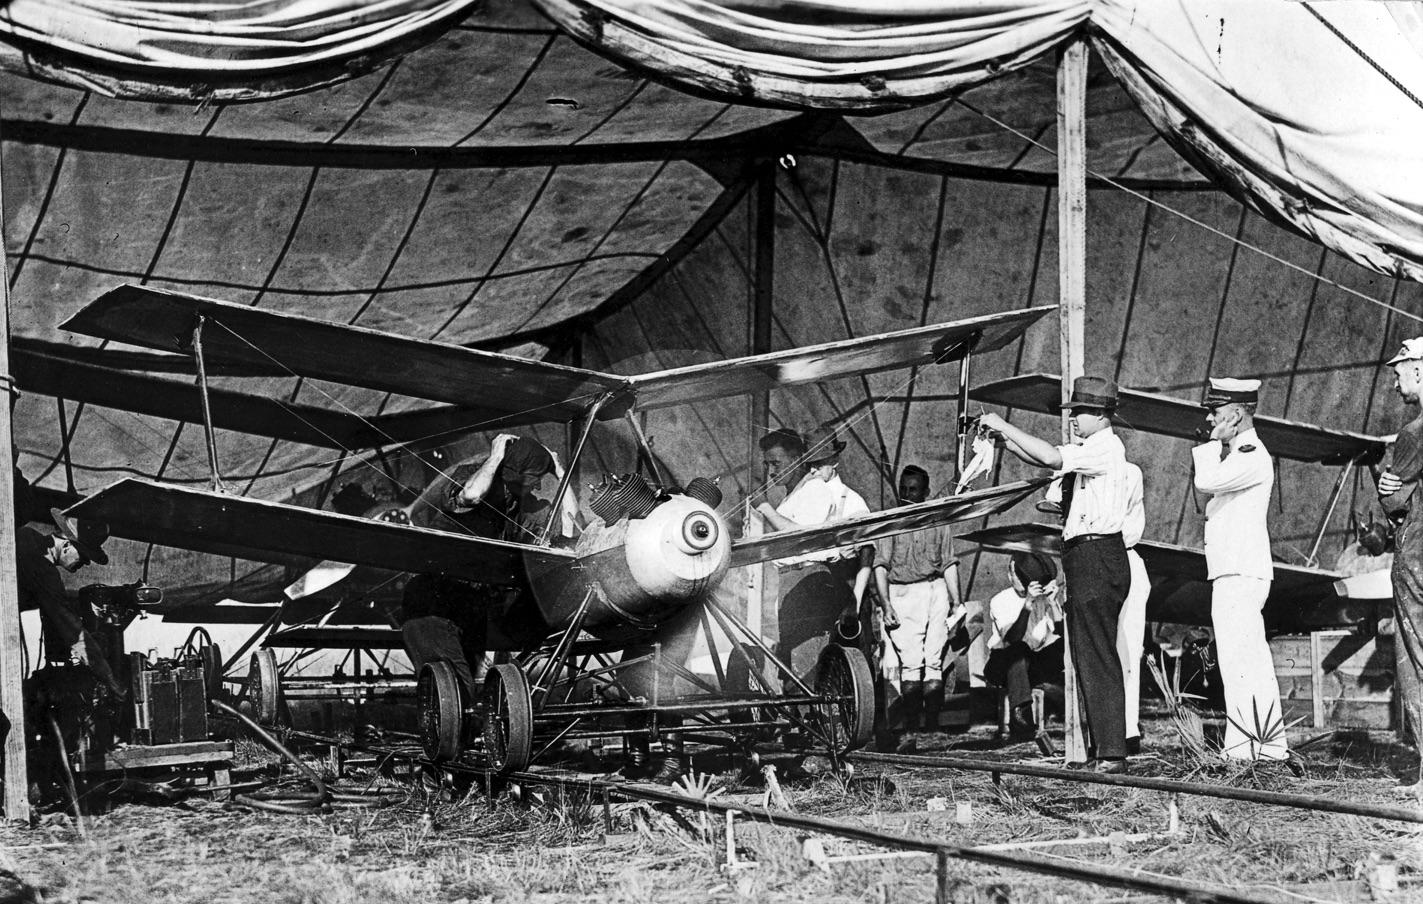
\includegraphics[width=0.3\textwidth,height=0.2\textwidth ]{figs/introducción/historia_drones/kettering-bug.jpg}
     \label{f:Kettering Bug}}
    \subfigure[Queen Bee]{
     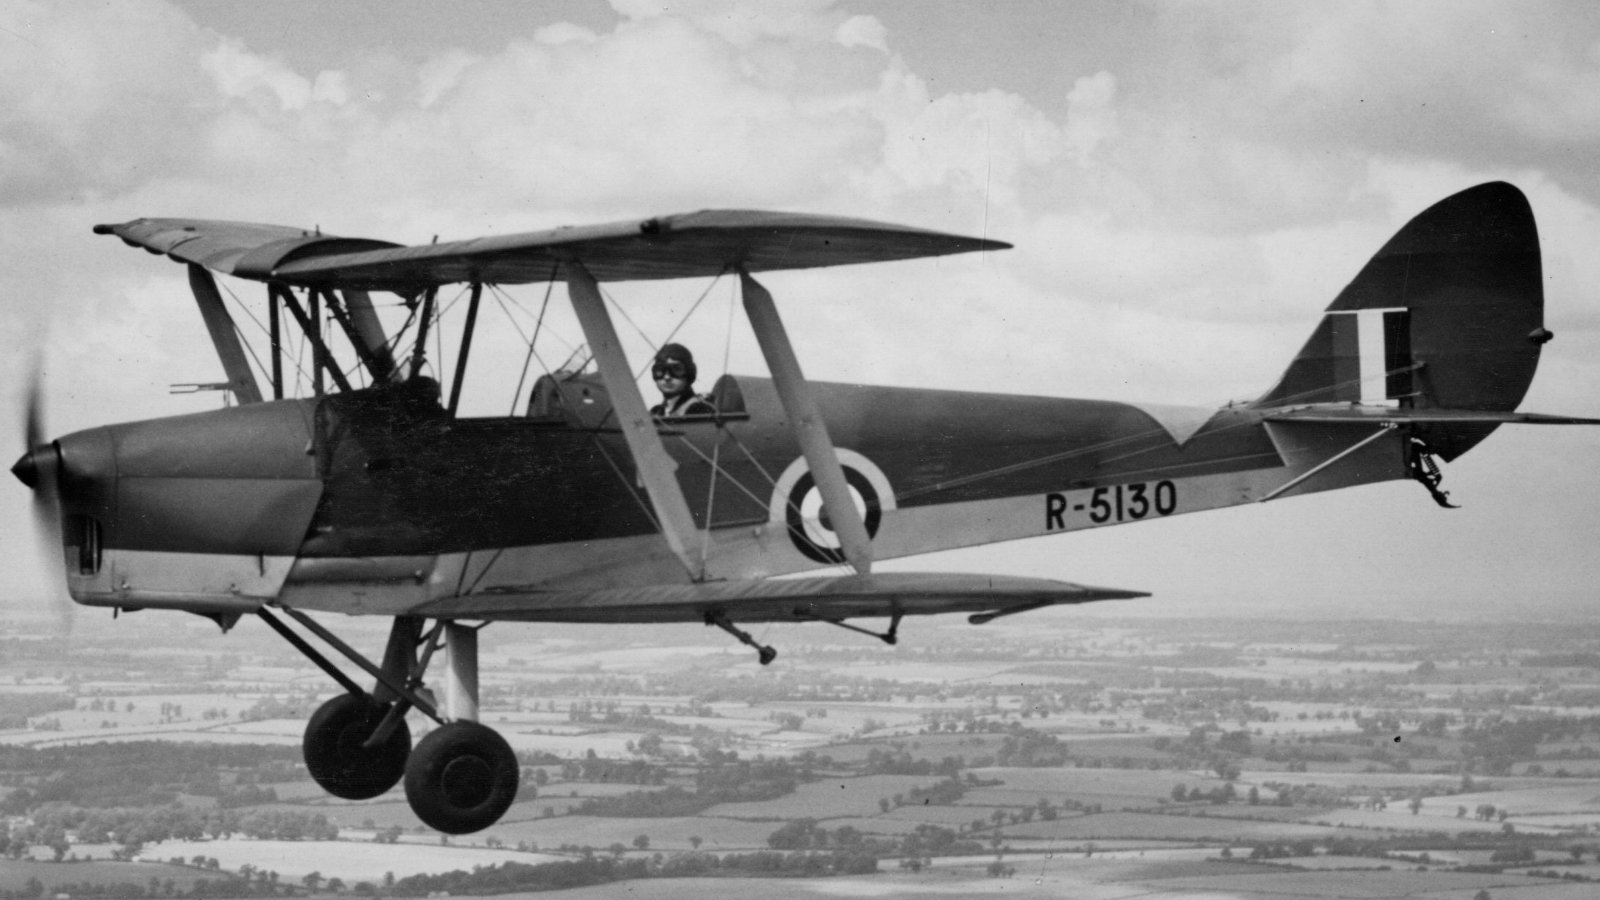
\includegraphics[width=0.3\textwidth,height=0.2\textwidth ]{figs/introducción/historia_drones/queen-bee.jpg}
     \label{f:Queen Bee}}
    \subfigure[V-1]{
      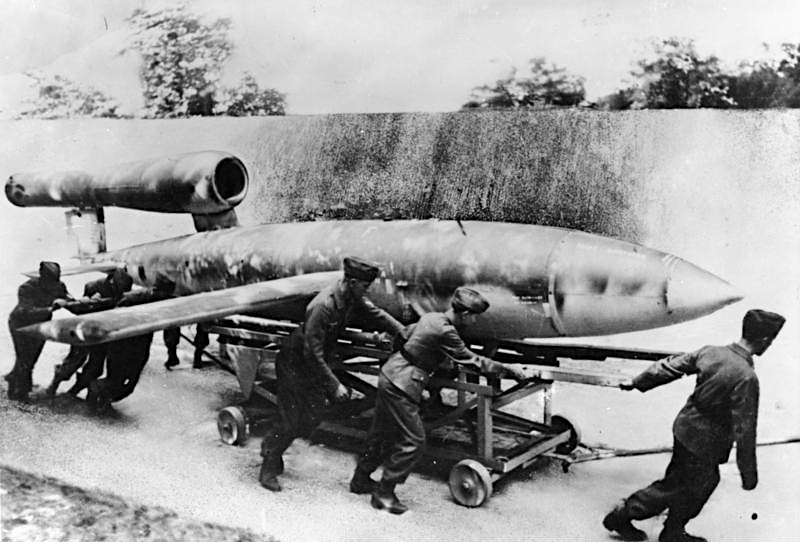
\includegraphics[width=0.3\textwidth,height=0.2\textwidth ]{figs/introducción/historia_drones/V-1.jpg}
      \label{f:V-1 "Flying Bomb"}}
    \subfigure[Proyect Aphrodite]{
      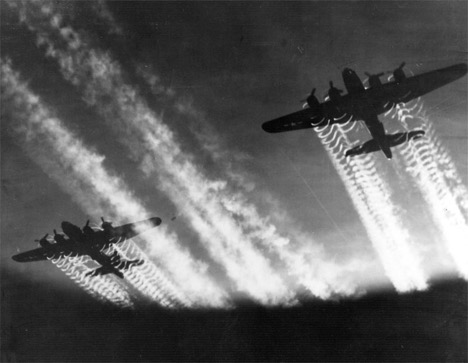
\includegraphics[width=0.3\textwidth,height=0.2\textwidth ]{figs/introducción/historia_drones/proyect-aphorite.jpg}
      \label{f:Proyect Aphrodite"}}
    \subfigure[Teledyne Ryan Firebee/Firefly]{
      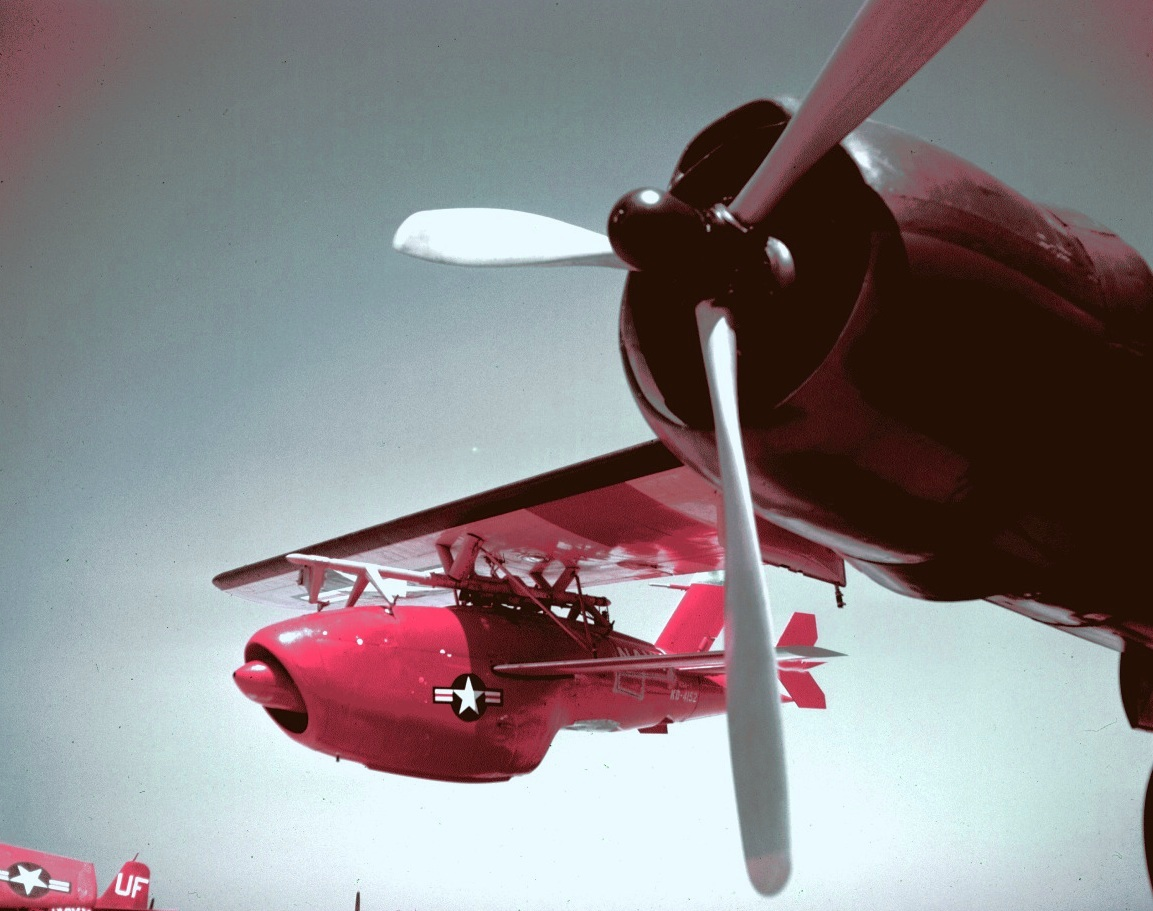
\includegraphics[width=0.3\textwidth,height=0.2\textwidth ]{figs/introducción/historia_drones/Firebee.jpg}
      \label{f:Teledyne Ryan Firebee/Firefly"}}
    \subfigure[Lockheed D-21]{
      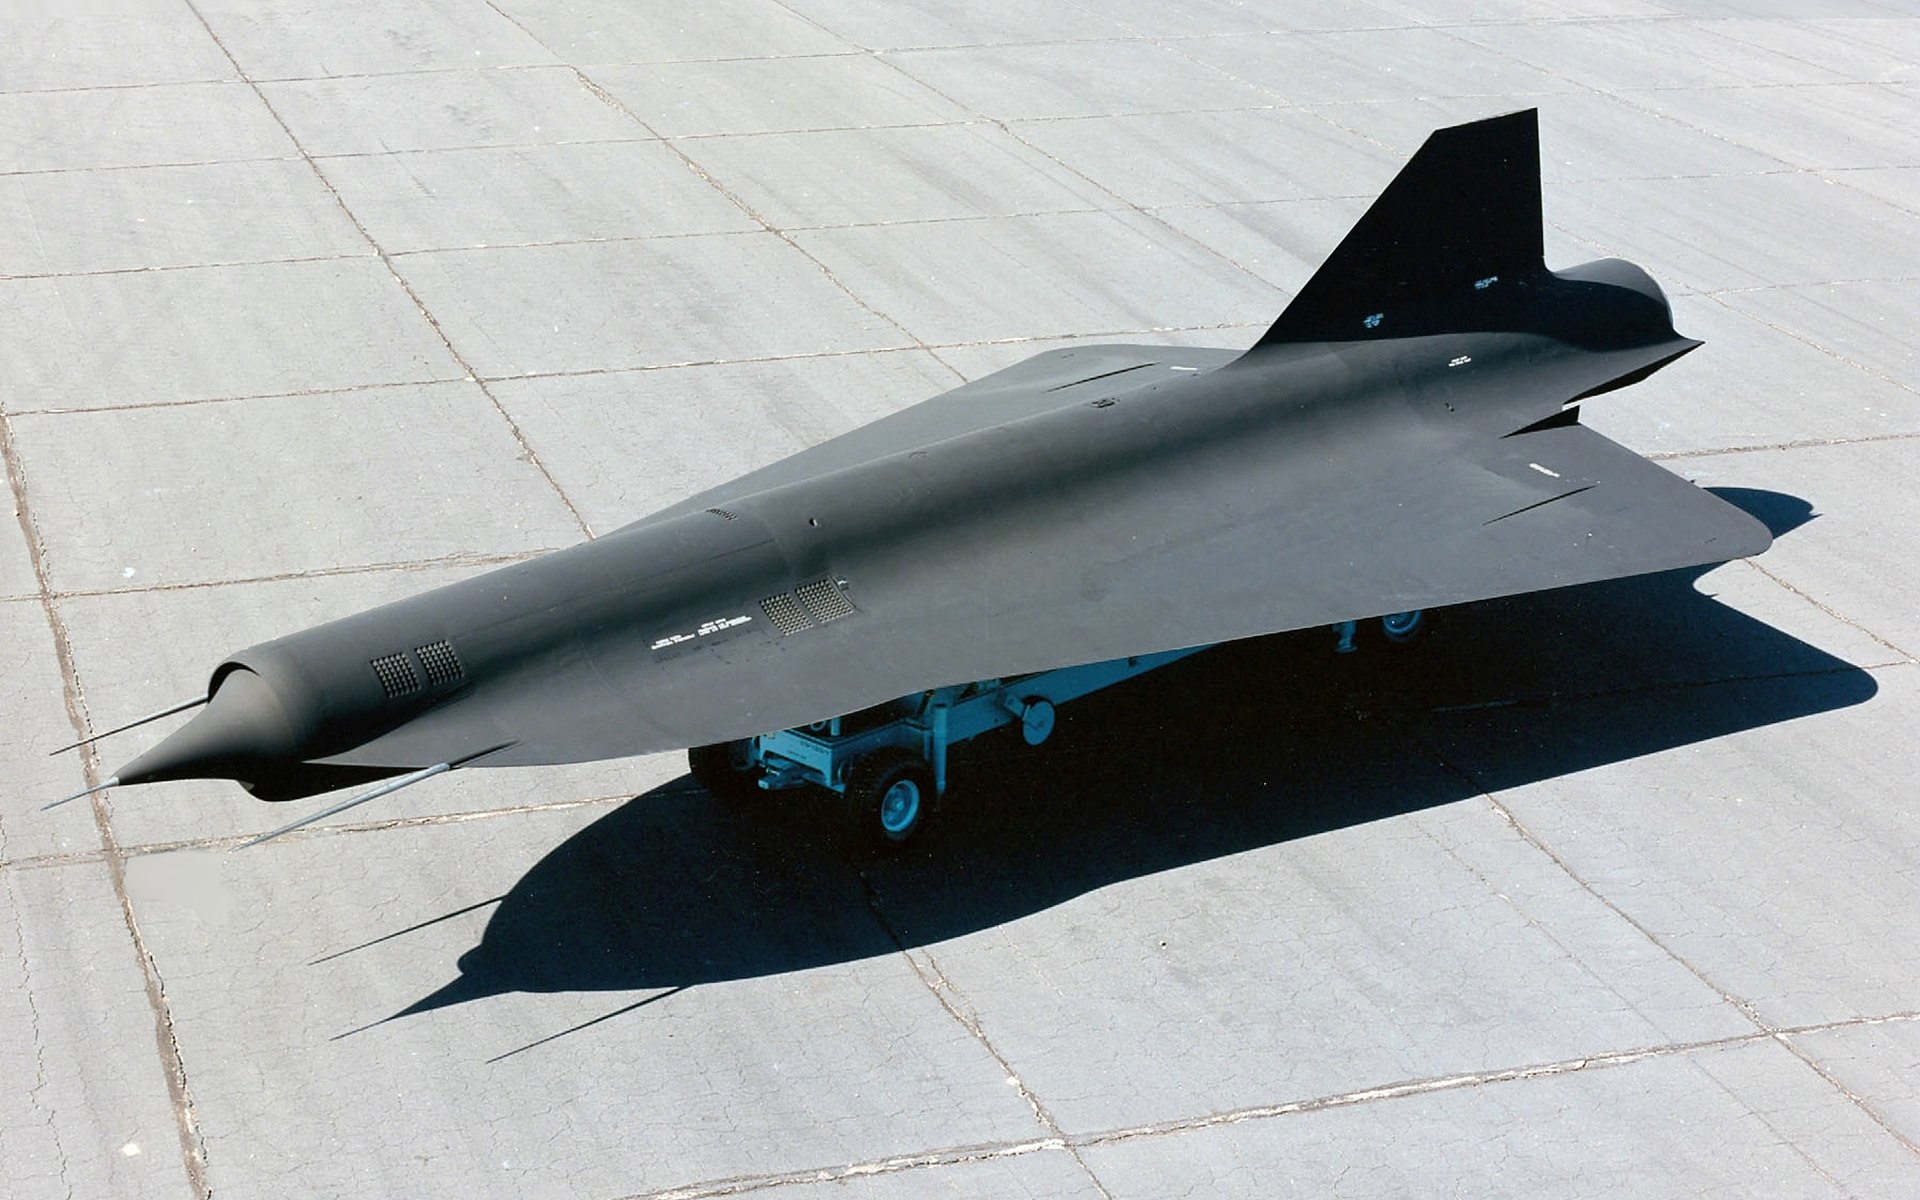
\includegraphics[width=0.3\textwidth,height=0.2\textwidth ]{figs/introducción/historia_drones/The_Lockheed_D-21.jpg}
      \label{f:Lockheed D-21"}}
    \subfigure[El Condor]{
      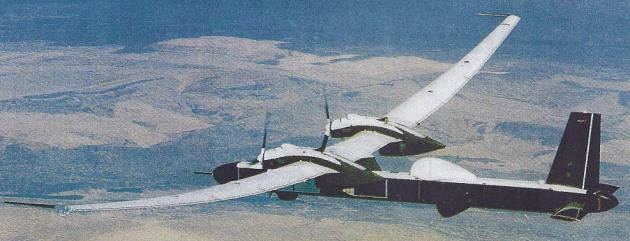
\includegraphics[width=0.3\textwidth,height=0.2\textwidth ]{figs/introducción/historia_drones/Boeing-Condor-UAV-23.png}
      \label{f:El Condor"}}
    \subfigure[Small UAV]{
      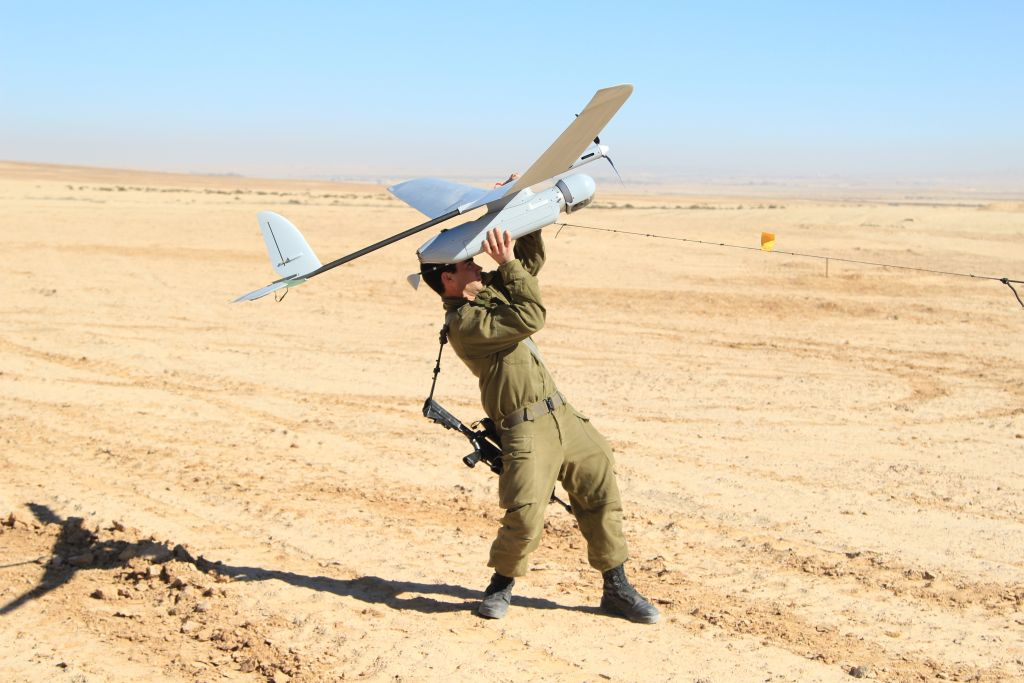
\includegraphics[width=0.3\textwidth,height=0.2\textwidth ]{figs/introducción/historia_drones/small-UAV.jpg}
      \label{f:small-UAV"}}
    \subfigure[Dron]{
      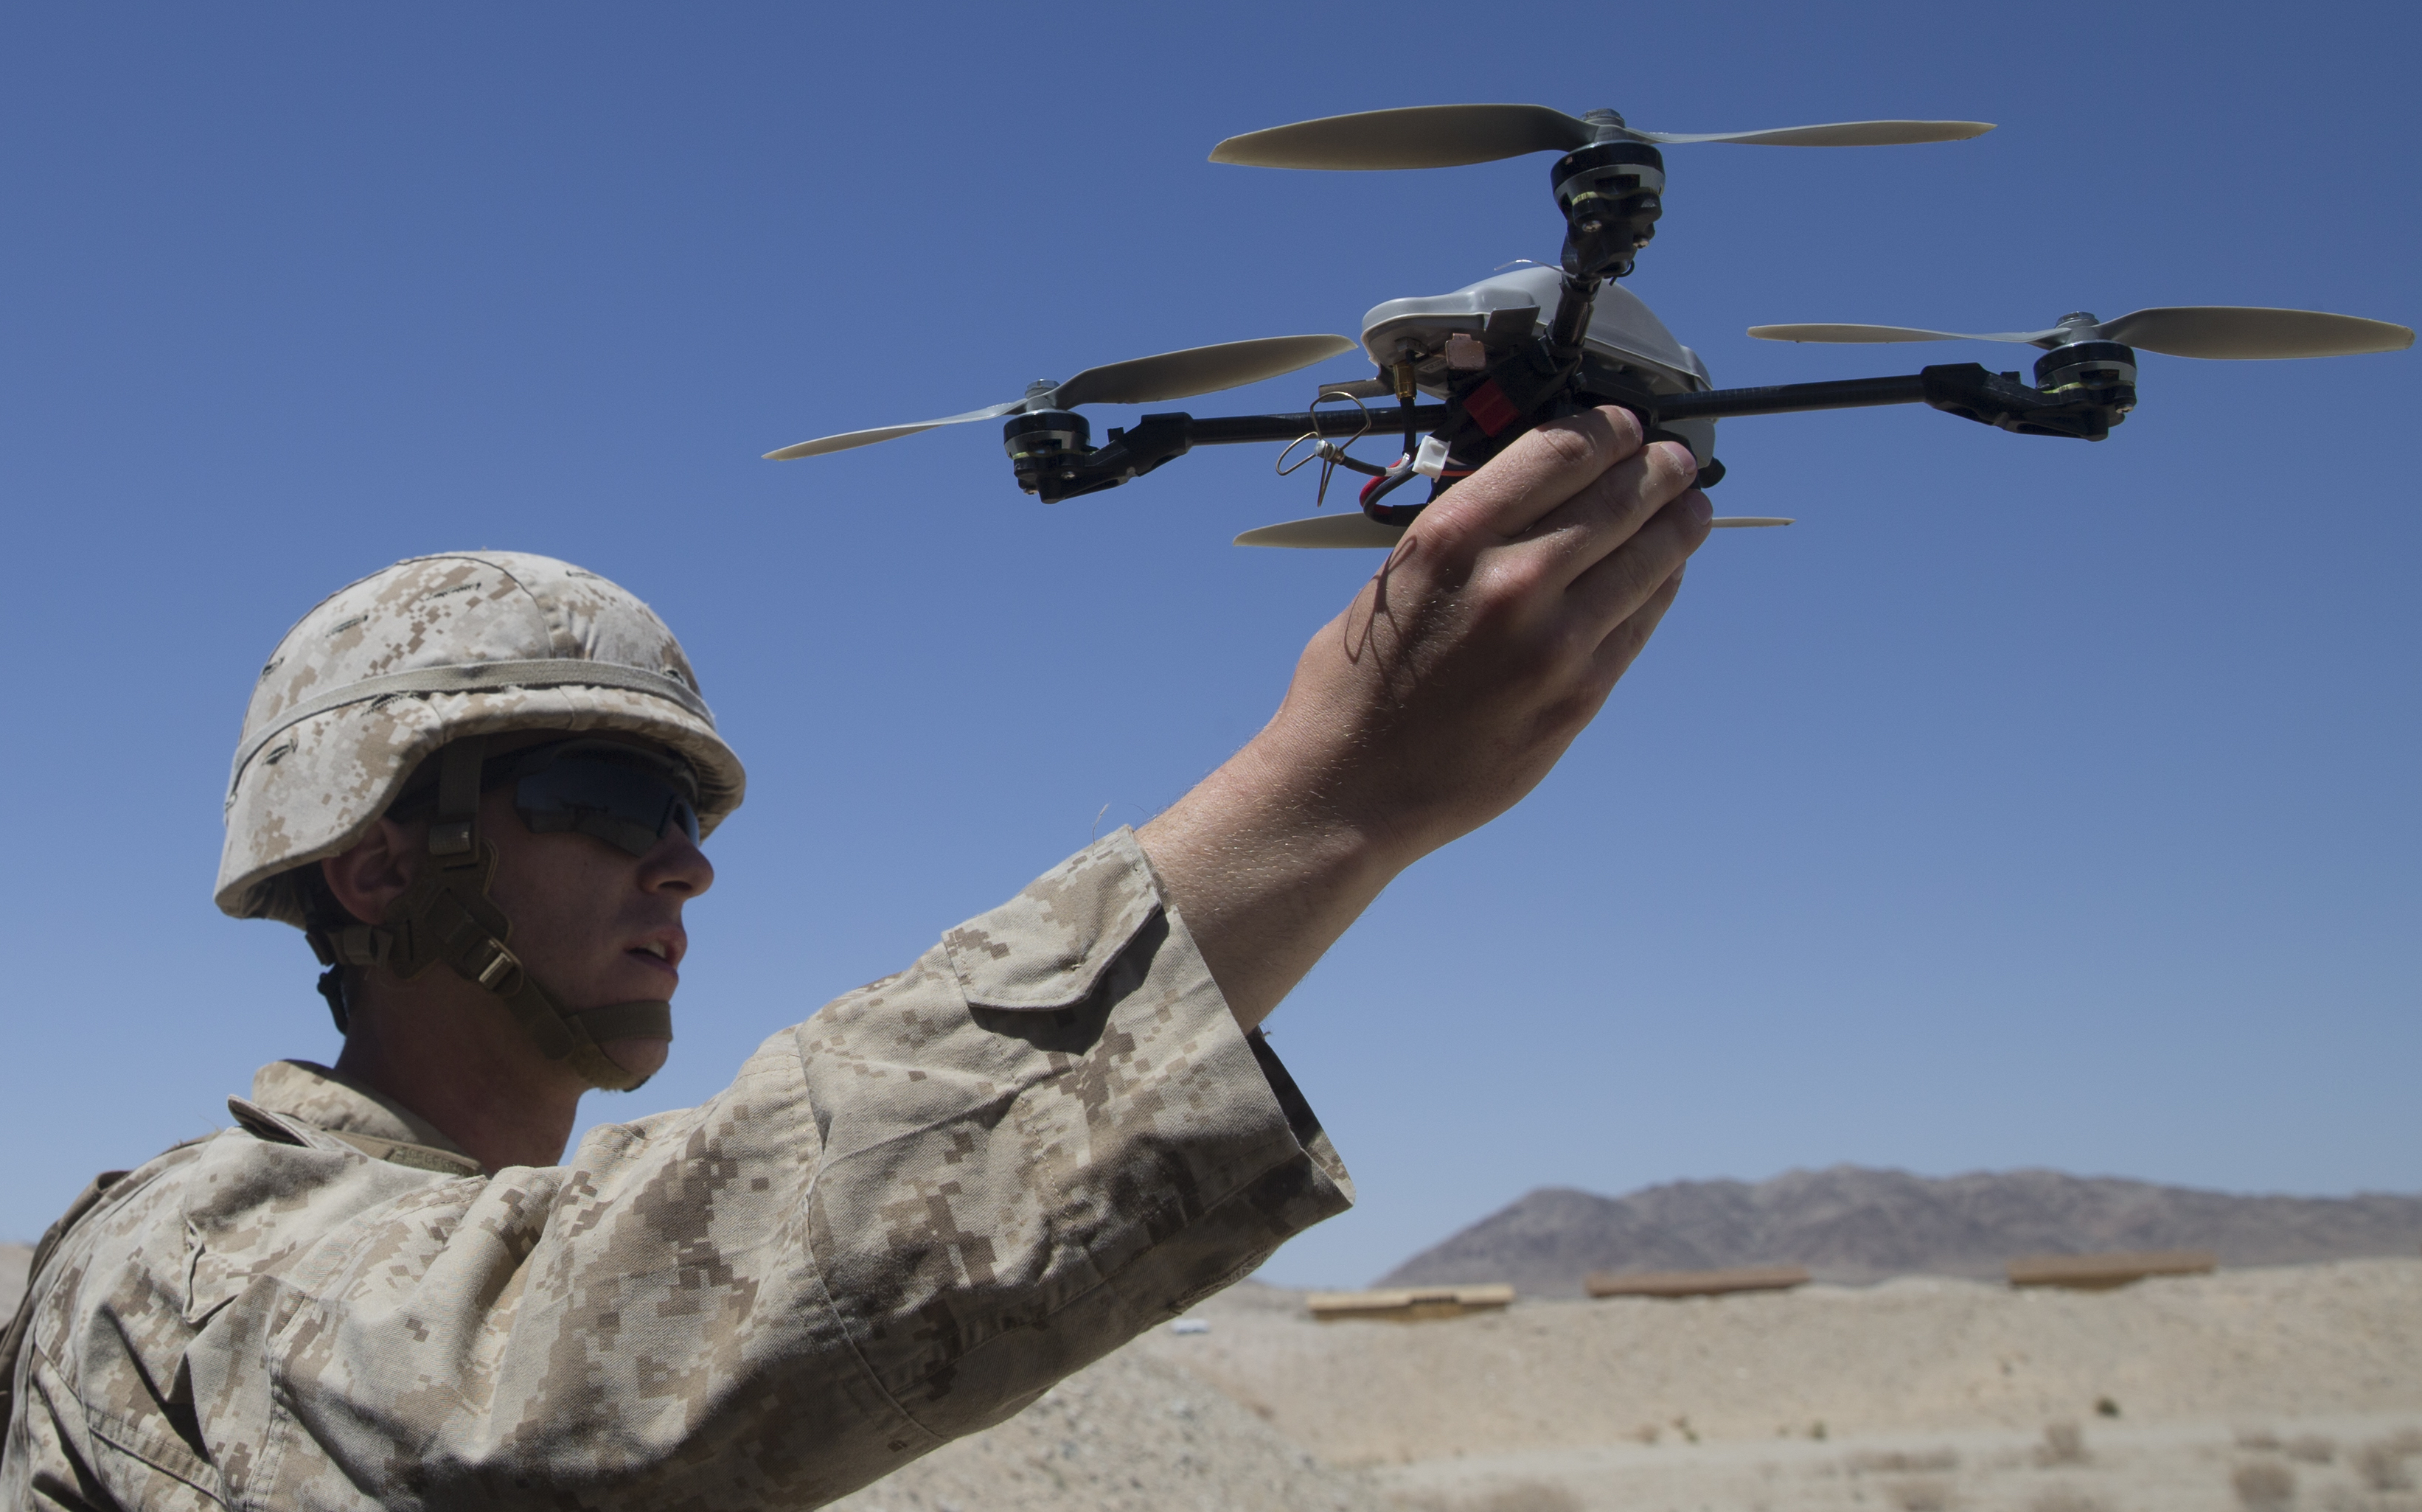
\includegraphics[width=0.3\textwidth,height=0.2\textwidth ]{figs/introducción/historia_drones/dron.jpg}
      \label{f:dron"}}
  \caption{Historia de los drones}
  \label{f:Drones}
  \end{center}
 \end{figure}

Cada vez es más común que los drones sean más sostificados y accesibles. Por ejemplo, el dron Ingenuity de la NASA se ha convertido en el primer vehículo aéreo autónomo en poder volar
sobre la superficie de otro planeta. Fue transportado a Marte mediante el rover Perseverance de la NASA, una vez fue posicionado el dron se elevó cerca de 3 metros realizando 
diferentes giros y desplazamientos tomando fotos a la superficie, teniendo la capacidad de escoger de forma autónoma los sitios de aterrizaje en el terreno marciano\footnote{\url{https://ciencia.nasa.gov/sistema-solar/finaliza-la-mision-del-helicoptero-ingenuity-en-marte/}}.
Este dron operaba de manera autónoma, controlado por sistemas de guía, navegación y control a bordo ejecutando los diferentes algoritmos desarrollados por la NASA. \newline

Uno de los grandes retos de este proyecto era demostrar la viabilidad del vuelo en la atmósfera de Marte, ya que su atmósfera esta compuesta por el 1\% de la densidad terrestre
dificultando el vuelo del dron. Sin embargo, gracias a su diseño ligero y a sus hélices especialmente diseñadas para crear suficiente sustentación en la atmósfera del planeta, el Ingenuity 
fue capaz de superar este desafío\footnote{\url{https://www.bbc.com/mundo/noticias-56738201}}. \newline
\begin{figure} [H]
  \begin{center}
    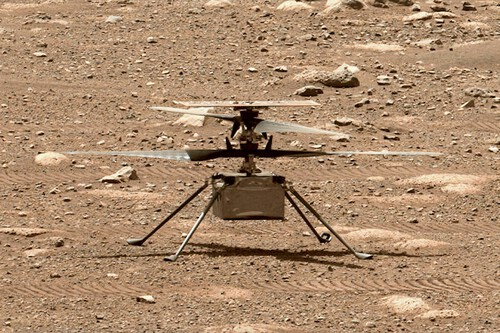
\includegraphics[scale=0.6]{figs/introducción/Ingenuity_II.jpeg}
  \end{center}
  \caption{El dron Ingenuity}
  \label{fig:Ingenuity}
\end{figure}\

Además, en su última fase, el Ingenuity realizó pruebas de vuelo experimentales para ampliar el conocimiento sobre cuáles eran sus límites aerodinámicos\footnote{\url{https://science.nasa.gov/mission/mars-2020-perseverance/ingenuity-mars-helicopter/}}.\newline

Otro ejemplo de uso de drones podemos tener el mantenimiento y control de redes eléctricas y otras infraestructuras. Algunas construcciones constan de grandes alturas y tamaños, lo que puede
dificultar el trabajo y su correcto mantenimiento. No obstante, estas tareas con los drones se agilizan y se vuelven más eficientes y robustas, porque permiten poder
inspeccionar dichas infraestructuras desde cerca sin poner en peligro a la seguridad de los operarios. 
Hay drones que se encargan en la monitorización de infraestructuras eléctricas. \newline

Unión Fenosa, la distribución eléctrica en España de Naturgy, en 2018 incorporó drones a sus instalaciones eléctricas para realizar labores de supervisión. Estos drones aportan 
soluciones optimizadas y eficientes en costes. Si tenemos en cuenta la longitud que puede tener las redes eléctricas, el uso de estos vehículos
autónomos facilita las tareas de supervisión equipados de cámaras de última generación permitiendo al operario observar en tiempo real el estado de las infraestructuras. Además de que los
drones podrían acceder a zonas de difícil acceso para comprobar daños y poder repararlos\footnote{\url{https://www.ufd.es/blog/primer-vuelo-de-un-dron-mas-alla-de-la-linea-visual/}}. \newline 


\begin{figure} [H]
  \begin{center}
    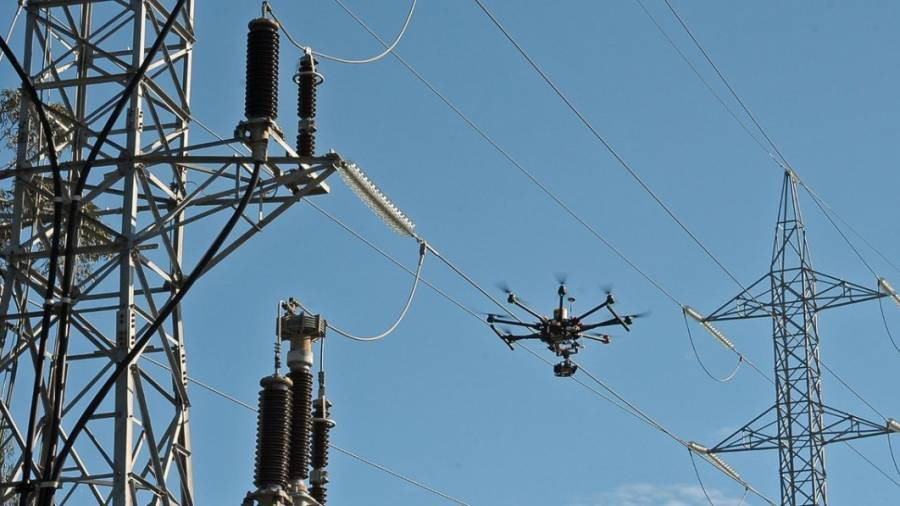
\includegraphics[scale=0.5]{figs/introducción/drones-red-electrica.jpg}
  \end{center}
  \caption{Drones en inspección eléctrica en Galicia}
  \label{fig:Fenosa}
\end{figure}\

Es importante mencionar que estos drones son teleoperados, lo que significa que requieren la intervención y el control directo de un operador humano para volar y realizar sus tareas 
de inspección y mantenimiento.\newline

Asimismo, Amazon ha estado trabajando en el desarrollo de drones autónomos para la entrega de paquetes durante varios años denominado así Prime Air\cite{AmazonPrimeAir}, 
que consiste en un sistema de entrega de paquetes utilizando estos vehículos. Durante este programa, han realizado diferentes pruebas de reparto de paquetes a clientes
en 60 minutos o menos. \newline

\begin{figure} [H]
  \begin{center}
    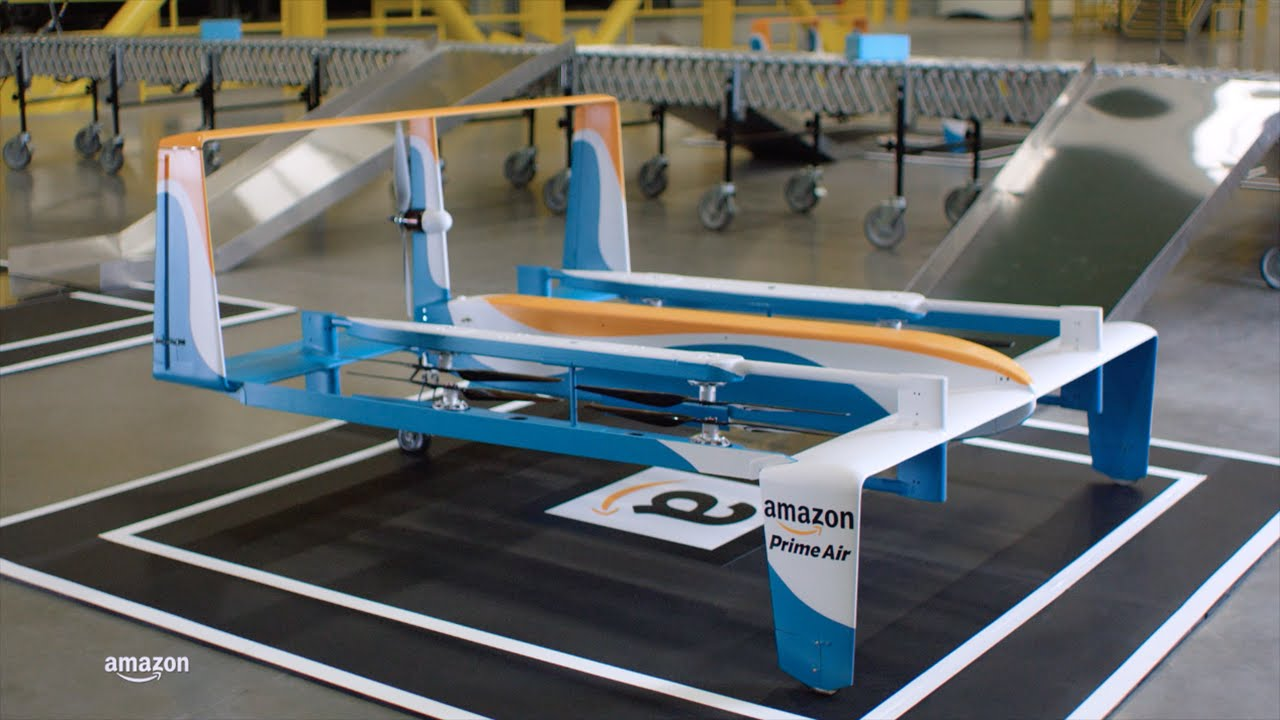
\includegraphics[scale=0.2]{figs/introducción/dron-amazon.jpg}
  \end{center}
  \caption{El primer prototipo de dron de Prime Air}
  \label{fig:PrimerPrimeAir}
\end{figure}\

A lo largo de los años, Amazon ha seguido investigando y diseñando nuevos modelos de drones como el dron autónomo MK27-2\footnote{\url{https://www.europapress.es/portaltic/gadgets/noticia-amazon-prime-air-comienza-entregar-pedidos-drones-estados-unidos-20221229115034.html}}. Fue el primer 
dron que utilizó Amazon para 
las primeras entregas dentro del programa Prime Air durante el año 2023, se basaba en un dron eléctrico capaz de entregar paquetes a los clientes en menos de una
hora y capaz de realizar vuelos evitando obstáculos como puede ser las chimeneas o las torres de telefonía aunque no puede realizar entregas durante tormentas, vientos fuertes, temperaturas
extremas o cualquier situación climatológica desfavorable. 

Este servicio solamente esta disponible para domicilios que tengan patios traseros que dispongan de espacio suficiente para que el dron pueda realizar el aterrizaje y la 
entrega del pedido.

\begin{figure} [H]
  \begin{center}
    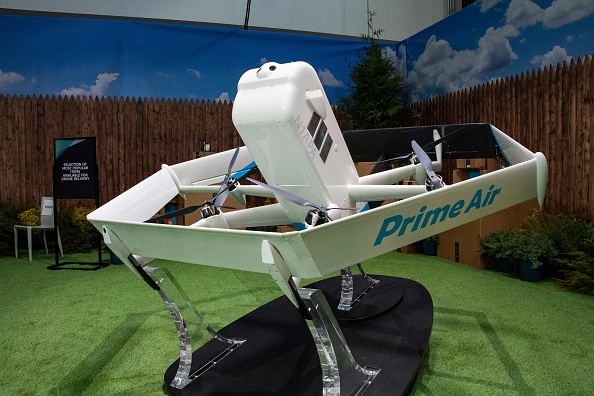
\includegraphics[scale=1.7]{figs/introducción/MK27-2.jpg}
  \end{center}
  \caption{El dron MK27-2}
  \label{fig:MK27-2}
\end{figure}\

Sin embargo, gracias al dron autónomo MK30 creado y diseñado por Amazon. Este pequeño dron será capaz de volar en diferentes condiciones climatológicas y 
constará de un sistema capaz de identificar y evitar obstáculos en el área de entrega. Una novedad de este dron en comparación con los anteriores modelos es que será capaz de aterrizar en espacios más reducidos lo que conlleva a que
este tipo de servicio pueda llegar a más vecindarios. \newline
Se tiene previsto que se llegue a probar en el año 2024 empezando por ciudades como Texas y California en Estados Unidos\footnote{\url{https://www.forbesargentina.com/innovacion/asi-nuevo-asombroso-dron-amazon-mk30-n42612}}. \newline

\begin{figure} [H]
  \begin{center}
    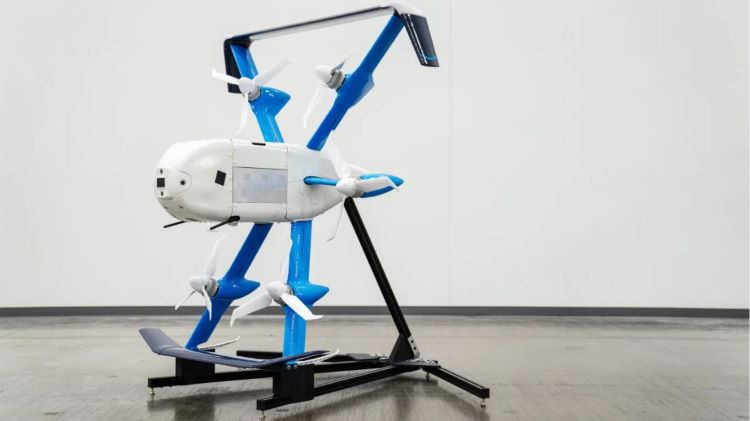
\includegraphics[scale=0.5]{figs/introducción/amazon-dron-mk30.jpg}
  \end{center}
  \caption{El dron MK30}
  \label{fig:MK30}
\end{figure}\

La navegación autónoma de drones sigue siendo un campo de investigación que busca permitir que los drones puedan volar de manera autónoma y segura.
Dentro de este ámbito, la detención y el seguimiento de carreteras se destacan como áreas prometedoras, un ejemplo de investigación sobre este campo, podemos 
tener este artículo \textit{Efficient Road Detection and Tracking for Unmmanned Aerial} \cite{article} que tiene como objetivo desarrollar un algoritmo de detección 
y seguimiento de carreteras específicas en videos capturados por vehículos aéreos no tripulados (UAV). Para la realizar la detección de carreteras utilizan 
un algoritmo denonimado Graph-Cut\footnote{\url{https://www.sciencedirect.com/topics/engineering/graph-cut-technique}}, 
que consiste en identificar y segmentar la imagen capturada por el dron para establecer la zona de interés,pero para obtener una segmentación más precisa y robusta de la carretera 
se combina con un modelo estadístico denonimado GMM\footnote{\url{https://builtin.com/articles/gaussian-mixture-model}} (Gaussian Mixture Model) para modelar las características de la imagen y representar regiones o clases
en la imagen (por ejemplo, carretera, fondo, vehículos).\newline

Una vez se realice la identificación de la carretera, se utilizará un algoritmo basado en homografía (tecnica geométrica), para ajustar la posición y la orientación del dron
en relación con la carretera. Este tipo de algoritmos de seguimiento de carreteras permite al dron seguir automáticamente las áreas que se definieron de la carretera. \newline

\begin{figure} [H]
  \begin{center}
    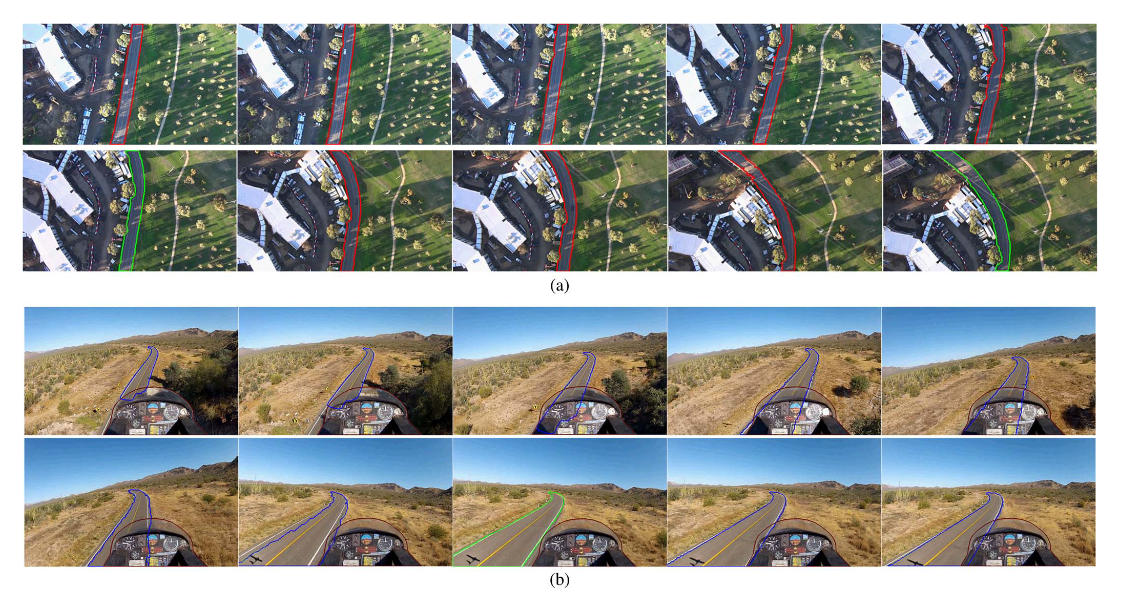
\includegraphics[scale=0.4]{figs/introducción/Efficient.png}
  \end{center}
  \caption{Resultados de detección y seguimiento de carreteras en Efficient Road Detection and Tracking for Unmmanned Aerial \cite{article}}
  \label{fig:Efficient}
\end{figure}\

Este enfoque puede tener aplicaciones como el monitoreo del tráfico y seguridad vial, seguimiento de vehículos terrestres o construcción de redes de carreteras para simulación. En un futuro cercano, puede que los drones sean más eficientes para las aplicaciones civiles y científicas incluyendo protección contra incendios forestales, misiones agrícolas, 
ayuda en catástrofes y más. 
Las demostraciones actuales del uso de los drones han revelado el potencial que pueden tener pero aun así el acceso al espacio aéreo sigue siendo un factor limitante. Con el paso del 
tiempo, se irá desarrollando nuevas tecnologías prácticas para poder permitir una integración segura en el espacio aéreo \cite{KrejciGarzon_2014}. \newline

En el artículo \textit{Automatic Damage Detection and Diagnosis for Hydraulic Structures Using Drones and Artificial Intelligence Techniques} \cite{rs15030615}, se explora el uso de drones
para monitorizar y diagnosticar daños estructurales en presas hidráulicas. El objetivo principal de este estudio es detectar y evaluar el estado de  grietas en estas estructuras. Para lograrlo, 
se emplean algoritmos de visión por computadora e inteligencia artificial. 
En particular, se utiliza una red neuronal llamada Xception \cite{Deeplabv3} junto con algoritmos de segmentación semántica de imágenes para detectar áreas afectadas. Los resultados experimentales, 
presentados en la figura \ref{fig:Hidraulica}, demuestran la eficacia de esta detección de daños en las presas hidráulicas mediante el uso de técnicas de visión e inteligencia artificial. 

\begin{figure} [H]
  \begin{center}
    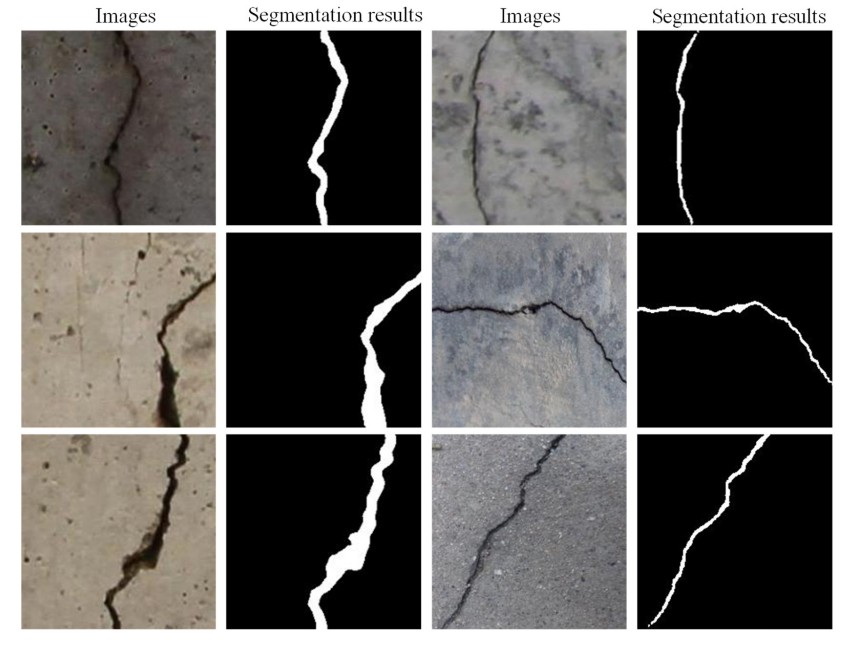
\includegraphics[scale=0.4]{figs/introducción/grietas.png}
  \end{center}
  \caption{ Demostración de la identificación de diferentes tipos de grietas \cite{Deeplabv3}}
  \label{fig:Hidraulica}
\end{figure}\

En resumen, los drones son una tecnología emergente con un potencial significativo
para transformar una variedad de industrias. Sin embargo, también plantean desafíos únicos que deben ser abordados a medida que se integran más plenamente en nuestra
sociedad. Con el desarrollo continuo de la tecnología de los drones y la evolución de las
regulaciones, es probable que veamos un aumento en la variedad de las aplicaciones de
los drones en el futuro. 


\section{La inteligencia artificial en la navegación autónoma de drones}
\label{sec:IA}

La incorporación de inteligencia artificial en el mundo de la robótica y en especial en los drones desempeña un papel crucial en la navegación autónoma, permitiéndoles tomar decisiones en tiempo real y adaptarse 
a entornos cambiantes de manera eficiente. Permitiendo a los drones poder aprender de sus experiencias y entender e interactuar con el entorno en el que se encuentran de una manera más
óptima. \newline

Los drones equipados con IA de percepción o de control pueden realizar vuelos de precisión, mantener la estabilidad incluso en condiciones adversas como fuertes vientos, y evitar obstáculos 
de forma dinámica. Esto es posible gracias a la combinación de datos sensoriales junto con los algoritmos de IA, lo que permite 
al dron interpretar su entorno y tomar decisiodecisiones en tiempo real. Uno de los enfoques más destacados en la navegación autónoma de drones es el aprendizaje automático. Este enfoque permite a los drones mejorar su objetivo a través de la experiencia 
y los datos recopilados durante el vuelo. 

\begin{figure} [H]
  \begin{center}
    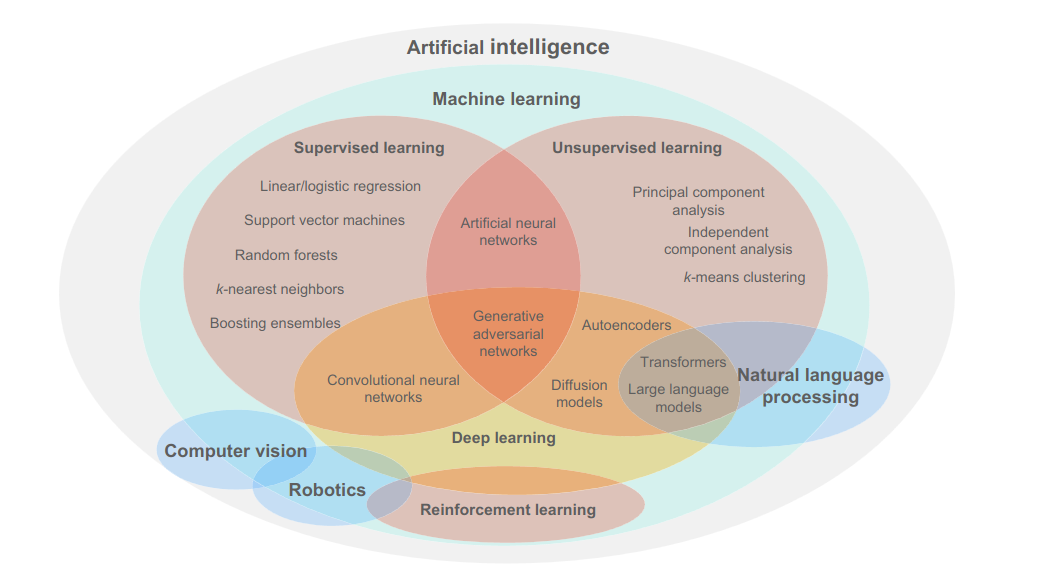
\includegraphics[scale=0.4]{figs/introducción/IA-diagrama.png}
  \end{center}
  \caption{Clasificación de Inteligencia Artificial \cite{IA}}
  \label{fig:ClasificaciónIA}
\end{figure}
\newpage

Por ejemplo, las CNN son capaces de analizar imágenes capturadas por las cámaras a bordo del dron para identificar obstáculos, 
peatones o vehículos. Un tipo de aplicación de uso de redes neuronales es la detección y clasificación de malas hierbas como se muestra 
en el artículo \textit{Weed detection and classification using UAVs and deep neural networks: mapping for localized treatment} \cite{CSIC}. Mediante el sensor de la cámara, el dron es capaz de capturar imágenes en tiempo real 
para más adelante usar la red neuronal CNN YOLOv8 \cite{Ultralytics_YOLOv8} para detectar y clasificar las diferentes hierbas que puede haber en un campo de cultivo. Este tipo de aplicación es bastante útil para la inspección
agrícola ya que los drones pueden crear mapas detallados que permiten a los agricultores aplicar herbicidas de manera más eficiente y precisa, también este tipo de aplicación puede
ser útil para tener una monitorización general sobre la salud del cultivo. El resultado se puede visualizar en la figura \ref{fig:malas hierbas}.\newline 

\begin{figure} [H]
  \begin{center}
    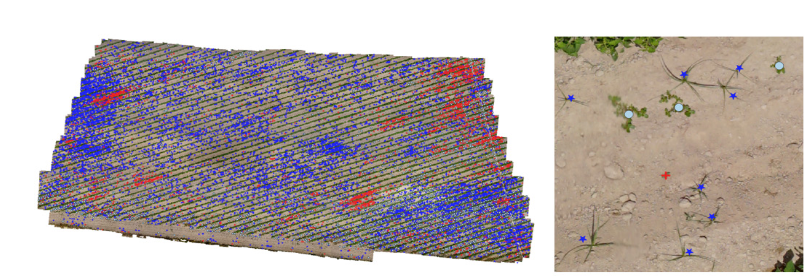
\includegraphics[scale=0.55]{figs/introducción/malashierbas.png}
  \end{center}
  \caption{Resultados de la detección y clasificación de malas hierbas en un cultivo \cite{CSIC}}
  \label{fig:malas hierbas}
\end{figure}

Por otro lado, reinforcement learning (RL) \cite{6025669} es una técnica dentro del aprendizaje automático que es interesante utilizar en la navegación autónoma de drones. Esta metodología permite
a los drones aprender a planificar rutas de forma autónoma, mejorando su desempeño a mediante un esquema de penalizaciones y recompensas permitiendo
así al dron poder tomar decisiones decisivas en situaciones puntuales. En el artículo \textit{Vision based drone obstacle avoidance by deep
reinforcement learning} \cite{ai2030023} precisamente se utiliza un algoritmo de RL para la evitación de obstáculos en un espacio continuo y se llega a conseguir que con estos
tipos de algoritmos que un dron pueda llegar aprender comportamientos y tomar decisiones por él mismo. 

\begin{figure} [H]
  \begin{center}
    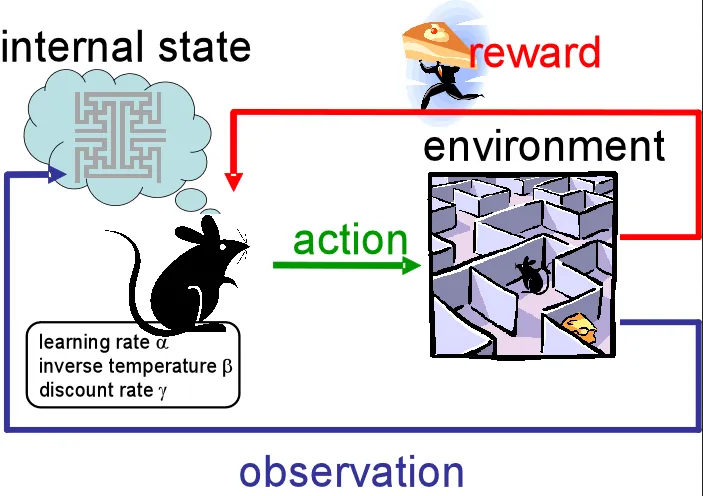
\includegraphics[scale=0.4]{figs/introducción/RL.png}
  \end{center}
  \caption{Esquema de Reinforcement Learning \cite{BecomingHuman_RL_Basics}}
  \label{fig:Reinforcement Learning}
\end{figure}\



En conclusión, la inteligencia artificial puede ser fundamental en la navegación autónoma de drones al permitirles percibir su entorno, podemos tomar decisiones y planificar acciones 
de manera anticipada y autónoma. A medida que vayamos avanzando, se espera que los drones tengan más sistemas de inteligencia artificial abordo para cubrir una amplia gama de tareas
de manera autónoma, lo que abriría nuevas fronteras en campos como el rescate, la vigilancia, la logística y la exploración, y que promete seguir transformando la forma en que 
interactuamos con el espacio aéreo en un futuro. 

\newpage
\section{Navegación autónoma en Airsim basada en inteligencia artificial y aprendizaje por refuerzo}
\label{sec:Navegación autónoma}

En este trabajo realizaremos un algoritmo basado en navegación autónoma para drones por entornos de carreteras sin intervención humana. Nuestro enfoque se basa en 
combinar la inteligencia artificial (IA) y aprendizaje por refuerzo (RL) para lograr vuelos autónomos y seguros, además de utilizar técnicas de procesamiento de imágenes 
y visión para detectar y segmentar las carreteras en las imágenes capturas por el dron permitiendo establecer regiones de interés específicas para la navegación 
autónoma.\newline

Este tipo de comportamientos pueden tener aplicaciones potenciales como monitorizar carreteras en la seguridad vial identificando los diferentes carriles de las carreteras y sus vehículos
en tiempo real, entrega de paquetes de manera autónoma siguiendo rutas de carreteras o vigilancia de accidentes en áreas de carreteras. \newline

En conclusión, con este trabajo de investigación buscamos impulsar el uso de la tecnología de drones en la seguiridad, planificación y eficiencia en el ámbito de las carreteras. 


